%----------------------------------------------------------------------------
%
%	This template was created by
%		Christian Krieg <christian.krieg@alumni.tuwien.ac.at>
%
%	April 2018
%
%----------------------------------------------------------------------------
%
\documentclass[%
	a4paper,
]
{article}
%
%----------------------------------------------------------------------------
%
% Institution
%
%\institution{Institute of Computer Technology}
%
%----------------------------------------------------------------------------
%
% Use the 'Libertine' font type
%
\usepackage{libertine}
\usepackage[T1]{fontenc}
\usepackage[utf8]{inputenc}
%
%----------------------------------------------------------------------------
%
% Set page margins
%
\usepackage{geometry}
\geometry{%
	left   = 2cm,
	right  = 2cm,
	top    = 2cm,
	bottom = 2cm
}
%
%----------------------------------------------------------------------------
%
% Set line spacing
%
\usepackage{setspace}
\setstretch{1}
%
%----------------------------------------------------------------------------
%
% Settings for hyperlinks
%
\usepackage{hyperref}
\hypersetup{%
	colorlinks = true,
	allcolors  = blue,
}
%
%----------------------------------------------------------------------------
%
% Use colors
%
\usepackage{xcolor}
\usepackage{colortbl}
%
%----------------------------------------------------------------------------
%
% Define a TODO and a DONE command
%
\newcommand{\todo}[1]{\textcolor{red}{#1}}
\newcommand{\done}[1]{}
%
%----------------------------------------------------------------------------
%
% Use glossaries
%
\usepackage{glossaries}
\makeglossaries
%
% Glossary entries
%
\newglossaryentry{fpga}{
	name = {FPGA},
	description = {Field-programmable gate array},
	text = {FPGA},
	first = {field-programmable gate array (FPGA)},
	plural = {FPGAs},
	firstplural = {field-programmable gate arrays (FPGAs)},
}
%
\newglossaryentry{trng}{
	name = {TRNG},
	description = {True-random number generator},
	text = {TRNG},
	first = {true-random number generator (TRNG)},
	plural = {TRNGs},
	firstplural = {true-random number generators (TRNGs)},
}
%
\newglossaryentry{bcd}{
  name={BCD},
  description={Binary-coded decimal},
  text={BCD},
  first={binary-coded decimal (BCD)},
}
%
\newglossaryentry{hdl}{
  name={HDL},
  description={Hardware description language},
  text={HDL},
  first={hardware description language (HDL)},
  plural={HDLs},
  firstplural={hardware description languages (HDLs)},
}

\newglossaryentry{lut}{
  name={LUT},
  description={Lookup Table},
  text={LUT},
  first={Specific Hardware in FPGAs to perform Lookup Table tasks},
  plural={LUTs},
  firstplural={Lookup Tables (LUTs)},
}
%
%\newglossaryentry{}{
%  name={},
%  description={},
%  text={},
%  first={},
%  plural={},
%  firstplural={},
%}
%
%----------------------------------------------------------------------------
%
% Settings for citations and the bibliography
%
\usepackage[%
	backend     = biber,
	maxbibnames = 99,
	autocite    = footnote,
	citestyle   = verbose-ibid,
	firstinits=true,
]{biblatex}
\bibliography{bib/report}
%
%----------------------------------------------------------------------------
%
%	TikZ -- TikZ ist kein Zeichenprogramm
%
\usepackage{tikz}
\usepackage{tikz-timing}
\usepackage{etoolbox}
\usetikzlibrary{mindmap}
\usetikzlibrary{shapes}
\usetikzlibrary{arrows}
\usetikzlibrary{decorations}
\usetikzlibrary{shapes.symbols}
\usetikzlibrary{shapes.geometric}
\usetikzlibrary{shapes.multipart}
\usetikzlibrary{positioning}
\usetikzlibrary{patterns}
\usetikzlibrary{calc}
\usetikzlibrary{scopes}         % cf. pgfmanual p.66
\usetikzlibrary{chains}         % cf. pgfmanual p.284
\usetikzlibrary{fit}
\usetikzlibrary{matrix}
\usetikzlibrary{decorations}
\usetikzlibrary{circuits.logic}
\usetikzlibrary{circuits.logic.IEC}
\usetikzlibrary{shapes.gates.logic.IEC}
\usetikzlibrary{circuits.logic.US}
\usetikzlibrary{shapes.gates.logic.US}
\usetikzlibrary{circuits.ee}
\usetikzlibrary{circuits.ee.IEC}
\usetikzlibrary{backgrounds}
\usetikzlibrary{automata}
\usetikzlibrary{intersections}
\usetikzlibrary{plotmarks}
\usepgflibrary{fpu}
\usetikzlibrary{decorations.pathreplacing}
%
%----------------------------------------------------------------------------
%
% TikZ shapes
%  
	% D flip-flops (DFFs) and shift register
% Author: Martin Scharrer
%\documentclass[a4paper,landscape]{article}

%\usepackage{pgf,tikz}
%%%<
%\usepackage{verbatim}
%\usepackage[active,tightpage]{preview}
%\PreviewEnvironment{tikzpicture}
%\setlength\PreviewBorder{5pt}%
%%%>

%\begin{comment}
%:Title: D flip-flops and shift register
%
%Example of a custom node shape for drawing  D flip-flops. The shape is used to draw a serial shift
%register. 
%
%\end{comment}
%
%\usetikzlibrary{calc,arrows}
%\usepackage{amsmath}
%\usepackage[left=1cm,right=1cm]{geometry}
%\pagestyle{empty}

\makeatletter

% Data Flip Flip (DFF) shape
\pgfdeclareshape{dff}{
  % The 'minimum width' and 'minimum height' keys, not the content, determine
  % the size
  \savedanchor\northeast{%
    \pgfmathsetlength\pgf@x{\pgfshapeminwidth}%
    \pgfmathsetlength\pgf@y{\pgfshapeminheight}%
    \pgf@x=0.5\pgf@x
    \pgf@y=0.5\pgf@y
  }
  % This is redundant, but makes some things easier:
  \savedanchor\southwest{%
    \pgfmathsetlength\pgf@x{\pgfshapeminwidth}%
    \pgfmathsetlength\pgf@y{\pgfshapeminheight}%
    \pgf@x=-0.5\pgf@x
    \pgf@y=-0.5\pgf@y
  }
  % Inherit from rectangle
  \inheritanchorborder[from=rectangle]

  % Define same anchor a normal rectangle has
  \anchor{center}{\pgfpointorigin}
  \anchor{north}{\northeast \pgf@x=0pt}
  \anchor{east}{\northeast \pgf@y=0pt}
  \anchor{south}{\southwest \pgf@x=0pt}
  \anchor{west}{\southwest \pgf@y=0pt}
  \anchor{north east}{\northeast}
  \anchor{north west}{\northeast \pgf@x=-\pgf@x}
  \anchor{south west}{\southwest}
  \anchor{south east}{\southwest \pgf@x=-\pgf@x}
  \anchor{text}{
    \pgfpointorigin
    \advance\pgf@x by -.5\wd\pgfnodeparttextbox%
    \advance\pgf@y by -.5\ht\pgfnodeparttextbox%
    \advance\pgf@y by +.5\dp\pgfnodeparttextbox%
  }

  % Define anchors for signal ports
  \anchor{D}{
    \pgf@process{\northeast}%
    \pgf@x=-1\pgf@x%
    \pgf@y=.5\pgf@y%
  }
  \anchor{CLK}{
    \pgf@process{\northeast}%
    \pgf@x=-1\pgf@x%
    \pgf@y=-.66666\pgf@y%
  }
  \anchor{CE}{
    \pgf@process{\northeast}%
    \pgf@x=-1\pgf@x%
    \pgf@y=-0.33333\pgf@y%
  }
  \anchor{Q}{
    \pgf@process{\northeast}%
    \pgf@y=.5\pgf@y%
  }
  \anchor{Qn}{
    \pgf@process{\northeast}%
    \pgf@y=-.5\pgf@y%
  }
  \anchor{R}{
    \pgf@process{\northeast}%
    \pgf@x=0pt%
  }
  \anchor{S}{
    \pgf@process{\northeast}%
    \pgf@x=0pt%
    \pgf@y=-\pgf@y%
  }
  % Draw the rectangle box and the port labels
  \backgroundpath{
    % Rectangle box
    \pgfpathrectanglecorners{\southwest}{\northeast}
    % Angle (>) for clock input
    \pgf@anchor@dff@CLK
    \pgf@xa=\pgf@x \pgf@ya=\pgf@y
    \pgf@xb=\pgf@x \pgf@yb=\pgf@y
    \pgf@xc=\pgf@x \pgf@yc=\pgf@y
    \pgfmathsetlength\pgf@x{.75ex} % size depends on font size
    \advance\pgf@ya by \pgf@x
    \advance\pgf@xb by \pgf@x
    \advance\pgf@yc by -\pgf@x
    \pgfpathmoveto{\pgfpoint{\pgf@xa}{\pgf@ya}}
    \pgfpathlineto{\pgfpoint{\pgf@xb}{\pgf@yb}}
    \pgfpathlineto{\pgfpoint{\pgf@xc}{\pgf@yc}}
    \pgfclosepath

    % Draw port labels
    \begingroup
    \tikzset{flip flop/port labels} % Use font from this style
    \tikz@textfont

    \pgf@anchor@dff@D
    \pgftext[left,base,at={\pgfpoint{\pgf@x}{\pgf@y}},x=\pgfshapeinnerxsep]{\raisebox{-0.75ex}{D}}

%    \pgf@anchor@dff@CE
%    \pgftext[left,base,at={\pgfpoint{\pgf@x}{\pgf@y}},x=\pgfshapeinnerxsep]{\raisebox{-0.75ex}{CE}}

    \pgf@anchor@dff@Q
    \pgftext[right,base,at={\pgfpoint{\pgf@x}{\pgf@y}},x=-\pgfshapeinnerxsep]{\raisebox{-.75ex}{Q}}

%    \pgf@anchor@dff@Qn
%    \pgftext[right,base,at={\pgfpoint{\pgf@x}{\pgf@y}},x=-\pgfshapeinnerxsep]{\raisebox{-.75ex}{$\overline{\mbox{Q}}$}}
%
%    \pgf@anchor@dff@R
%    \pgftext[top,at={\pgfpoint{\pgf@x}{\pgf@y}},y=-\pgfshapeinnerysep]{R}
%
%    \pgf@anchor@dff@S
%    \pgftext[bottom,at={\pgfpoint{\pgf@x}{\pgf@y}},y=\pgfshapeinnerysep]{S}
    \endgroup
  }
}

% Key to add font macros to the current font
\tikzset{add font/.code={\expandafter\def\expandafter\tikz@textfont\expandafter{\tikz@textfont#1}}} 

% Define default style for this node
% \tikzset{flip flop/port labels/.style={font=\sffamily\scriptsize}}
%\tikzset{every dff node/.style={draw,minimum width=2cm,minimum 
%height=2.828427125cm,very thick,inner sep=1mm,outer sep=0pt,cap=round,add 
%font=\sffamily}}
\tikzset{flip flop/port labels/.style={font=\tiny}}
\tikzset{every dff node/.style={draw,minimum width=.75cm,minimum 
height=1cm,inner sep=1mm,outer sep=0pt,cap=round,font=\scriptsize}}

\makeatother

%\begin{document}
%
%\begin{tikzpicture}[font=\sffamily,>=triangle 45]
%  \def\N{7}  % Number of Flip-Flops minus one
%
%  % Place FFs
%  \foreach \m in {0,...,\N}
%    \node [shape=dff] (DFF\m) at ($ 3*(\m,0) $) {Bit \#\m};
%
%  % Connect FFs (Q1 with D1, etc.)
%  \def\p{0}  % Used to save the previous number
%  \foreach \m in {1,...,\N} { % Note that it starts with 1, not 0
%    \draw [->] (DFF\p.Q) -- (DFF\m.D);
%    \global\let\p\m
%  }
%
%  % Connect and label data in- and output port
%  \draw [<-] (DFF0.D) -- +(-1,0) node [anchor=east] {input} ;
%  \draw [->] (DFF\N.Q) -- +(1,0) node [anchor=west] {output};
%
%  % 'Reset' port label
%  \path (DFF0) +(-2cm,+2cm) coordinate (temp)
%    node [anchor=east] {reset};
%  % Connect resets
%  \foreach \m in {0,...,\N}
%    \draw [->] (temp) -| (DFF\m.R);
%
%  % 'Set' port label
%  \path (DFF0) +(-2cm,-2cm) coordinate (temp)
%    node [anchor=east] {set};
%  % Connect sets
%  \foreach \m in {0,...,\N}
%    \draw [->] (temp) -| (DFF\m.S);
%
%  % Clock port label
%  \path (DFF0) +(-2cm,-2.5cm) coordinate (temp)
%    node [anchor=east] {clock};
%  \foreach \m in {0,...,\N}
%    \draw [->] (temp) -| ($ (DFF\m.CLK) + (-5mm,0) $) --(DFF\m.CLK);
%
%  % Clock port label
%  \path (DFF0) +(-2cm,-3cm) coordinate (temp)
%    node [anchor=east] {clock enable};
%  \foreach \m in {0,...,\N}
%    \draw [->] (temp) -| ($ (DFF\m.CE) + (-7.5mm,0) $) --(DFF\m.CE);
%\end{tikzpicture}
%
%\end{document}

%
%----------------------------------------------------------------------------
%
% Use AMS math fonts
%
\usepackage{amsfonts}
\usepackage[sans]{dsfont}
%
%----------------------------------------------------------------------------
%
% Use multiple figures in one float
%
\usepackage{subcaption}
%
%----------------------------------------------------------------------------
%
% Use dummy text
%
\usepackage{lipsum}
%
%----------------------------------------------------------------------------
%
% Use extended list environments (e.g., 'inparaenum')
%
\usepackage{paralist}
%
%----------------------------------------------------------------------------
%
% Use listings
%
\usepackage{listings}

\lstdefinestyle{vhdl}
{
	language=VHDL,
  basicstyle=\linespread{1}\scriptsize\ttfamily\color{black},
  commentstyle=\scriptsize\itshape,
  escapeinside={(*@}{@*)},
  frame=single, numbers=left,
%  numbersep=5pt,
  xleftmargin=15pt,
  xrightmargin=5pt,
  numbersep=5pt,
  breaklines=true,
  moredelim=**[is][\ttfamily\bfseries\color{red}]{(*}{*)},
}

\lstdefinestyle{verilog}
{
	language=Verilog,
  basicstyle=\linespread{1}\scriptsize\ttfamily\color{black},
  commentstyle=\scriptsize\itshape,
  escapeinside={(*@}{@*)},
  frame=single, numbers=left,
%  numbersep=5pt,
  xleftmargin=15pt,
  xrightmargin=5pt,
  numbersep=5pt,
  breaklines=true,
  moredelim=**[is][\ttfamily\bfseries\color{red}]{(*}{*)},
}
%
%----------------------------------------------------------------------------
%
% Typeset pseudo code
%
\usepackage{syntax}
%
%----------------------------------------------------------------------------
%
% More options for boxes
%
\usepackage{realboxes}
%
% Command for vertical text in tabulars
%
\newcommand*\rot{\rotatebox{90}}
%
%----------------------------------------------------------------------------
%
% Use \textsubscript
%
\usepackage{fixltx2e}
%
%----------------------------------------------------------------------------
%
% More options for tabulars
%
\usepackage{array}
%
%----------------------------------------------------------------------------
%
% Use appendices
%
\usepackage[titletoc]{appendix}
%
%----------------------------------------------------------------------------
%
% Use the cleverref package -- Load this package as the very last!
%
\usepackage{cleveref}
%
%----------------------------------------------------------------------------
%
%
%----------------------------------------------------------------------------
%
% Document body
%
\begin{document}
%
%----------------------------------------------------------------------------
%
\begin{titlepage}

	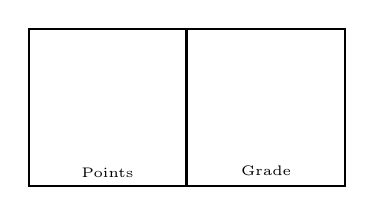
\begin{tikzpicture}[thick]
		\node (points) at (0,0) [draw,minimum size=2cm] {};
		\node (lbl-points) at (points.south) [anchor=south,font=\tiny] {Points};
		\node (grade) at (points.east) [draw,minimum size=2cm,anchor=west,
			outer sep=0] {};
		\node (lbl-grade) at (grade.south) [anchor=south,font=\tiny] {Grade};
	\end{tikzpicture}

	\begin{flushright}

		% Update this with your team number
		\huge\bfseries
		Team: 6 \\[1em]

		% Update this with your matriculation number, first name, second name
		\large
		01228774 Constantin SCHIEBER \#1	\\
		0122576 Petar KOSIC \#2	\\
	
	\end{flushright}

	\vspace{5em}

	\begin{center}
		{\huge Digital Integrated Circuits Lab (LDIS)}\\[1em]
		{\Large 384.088, Summer Term 2018} \\[2em]
		{\large Supervisors:\\[.5em]
			Christian Krieg, Martin Mosbeck, Axel Jantsch} \\[10em]

		{\Huge Task 1: Implementing a TRNG on a FPGA}\\[10em]
	\end{center}


	\begin{abstract}

		Parts of a key derivation function (KDF) - Argon2 - had to be implemented and integrated
with implementations of other groups. The result of this task is a working KDF that can be
reused.

A Permutation function, a compression function and a truncation function and the
verification process are subsequently presented in this work.


	\end{abstract}

\end{titlepage}
%
%----------------------------------------------------------------------------
%
\section{Problem statement and motivation}
\label{sec:problem}

A \gls{trng} based on the paper from \autocite{Majzoobi2011} had to be implemented.

The paper shows an approach that promises a resource efficient and fast solution to the
problem of generating long enough keys for cryptographic algorithms. The reproduction of
the results in the paper is a challenging and important task, as the paper is very
incomplete regarding information about the actual implementation.

The source of randomness is based on the metastability characteristics of a d-flipflop when violating setup or hold times of the flipflop.
To create such violations the novel approach of delay lines is introduced. The data and
clock input ports of the flipflop are both preceded by a series of \glspl{lut} blocks. 
These \glspl{lut} blocks are functionally just used as inverters - but due to the
inner structe of a \glspl{lut} a delay can be introduced by applying different control
signals to the \glspl{lut} ports.


%
%----------------------------------------------------------------------------
%
\section{Implementation (proposed solution)}
\label{sec:solution}

A naive implementation of the papers approach did not lead to any reproduceable output.
Therefore a list of stepstones that were encountered while working on a solution is
compiled. The most important takeway from the following is that the top and bottom delay
lines need to be symmetric in terms of placement, routing and ports.

The paper authors omit any details on the actual implementation, but as this 
question in the comments of a blog post (most likely from the paper author) shows it was
of interest for them as well \autocite{Mehrdad2010} and that they also struggled with
optimization during synthesis.

The following constraints provide us with a solid ground for further work as placement,
routing and pin assignments are now mostly consistent with every synthesis run. 

\subsection{Unwanted Optimization of Logic Elements}
This was mainly a problem for the \gls{lut} blocks and sometimes a problem for
the d-flipflop. The synthesis tool tries to minimize the use of \gls{lut} blocks as it
rightfully detects the redundancy in the logic. It therefore minimizes the LUT6 (6 inputs)
blocks to combinations of smaller LUT Blocks - controlling the delay is therefore not
possible anymore (on the one hand due to the missing delay of the mutliplexers in the lut
and on the other hand due to the possible asymmetry in the top and bottom delay paths).

\subsubsection{Mitigation}
The Xilinx / Vivado Documentation states on this topic that the DONT_TOUCH attribute is
the best option \autocite{XilinxAttributes}. It should ensure that the signal is kept, in
reality this does not work reliably, or the author didn't understand it fully. 

\begin{lstlisting}[
	style = vhdl,
	caption = {Attribute Declaration in VHDL, for the flipflop},
	label = lst:attrDontTouch,
]
	attribute DONT_TOUCH : string;
	attribute DONT_TOUCH of flipflop: label is "TRUE";
\end{lstlisting}

\subsection{Unwanted Optimization of Logic Element Placement}
The luts would be placed in many different ways for every synthesis run, even if nothing
else changed. Fixing the location of the luts to specific slices solved this problem.
A spreadsheet was created to ease the creation of the assignments.

\subsubsection{Mitigation}
\begin{lstlisting}[
	style = vhdl,
	caption = {Set location of a lut},
	label = lst:setLoc,
]
set_property LOC SLICE_X85Y125 [get_cells gen_bot_coarse_plds[1].i_bot_coarse_pld/g0_b0]
\end{lstlisting}

 
\subsection{Unwanted Optimization of Routing Paths}
As the routing tool is - rightfully - trying to minimize setup and hold times in the
routed design it creates asymmetric paths with delays that can be longer than the
logic delay introduced by the lut blocks. Net Delays of up to 126ns could be observed,
while the logic delay on the same path would only account for 7ns. 
This in itself would not cause a problem if the top and bottom path would show the same
delay. But already a 5\% deviation of top and bottom path would render the delay of
the delay lines useless.

\subsubsection{Mitigation}
Timing analysis and optimization can be disabled for net paths or cells. For the sake of
simplicity all cells in in the delay path very excluded from the timing analysis.
This lead to more direct and more consistent routings. 

\begin{lstlisting}[
	style = vhdl,
	caption = {Disable the timing analysis for luts},
	label = lst:disableTiming,
	]
set_disable_timing [get_cells {gen_top_coarse_plds[*].i_top_coarse_pld/g0_b0}]
set_disable_timing [get_cells {gen_top_fine_plds[*].i_top_fine_pld/g0_b0}]

set_disable_timing [get_cells {gen_bot_coarse_plds[*].i_bot_coarse_pld/g0_b0}]
set_disable_timing [get_cells {gen_bot_fine_plds[*].i_bot_fine_pld/g0_b0}]
\end{lstlisting}

Another option that has to be considered is to route the delay path nets first and only
after that the rest. No specific improvements could be obsereved, alltough other groups
reported some.

\begin{lstlisting}[
	style = vhdl,
	caption = {Route critical nets first},
	label = lst:routeFirst,
	]
set preRoutes [get_nets  {*lut_t_* *lut_b_*}]
route_design -net [get_nets \$preRoutes] -delay
route_design -preserve
\end{lstlisting}

\subsection{Unwanted Optimization of Port Elements}
The synthesis / routing tool can decide how to arrange the port mapping of the luts, e.g.
port A6 of the lut can be mapped to signal I0 while the expected mapping would be A0:I0. 
This again causes asymmetry in the delay paths as certain ports (with A6 being the fastest
and A0 the slowest) of the lut react faster than others (as per the design of the lut).

\subsubsection{Mitigation}
Ports of logic elements can be fixed by the following commands. 

\begin{lstlisting}[
	style = vhdl,
	caption = {Disable the timing analysis for luts},
	label = lst:disableTiming,
	]
set_property LOCK_PINS { I0:A1 I1:A2 I2:A3 I3:A4 I4:A5 I5:A6 } [get_cells *i_top_coarse_pld/g0_b0 ]
set_property LOCK_PINS { I0:A1 I1:A2 I2:A3 I3:A4 I4:A5 I5:A6 } [get_cells *i_top_fine_pld/g0_b0 ]
set_property LOCK_PINS { I0:A1 I1:A2 I2:A3 I3:A4 I4:A5 I5:A6 } [get_cells *i_bot_coarse_pld/g0_b0 ]
set_property LOCK_PINS { I0:A1 I1:A2 I2:A3 I3:A4 I4:A5 I5:A6 } [get_cells *i_bot_fine_pld/g0_b0 ]
\end{lstlisting}



\subsection{Top Module State Machine}
For the main implementation we used a state machine for all the logic. \\\\
STATE_UART_WELCOME:\\
The Logic starts in STATE_UART_WELCOME, which sends an welcome message to the user via UART. Afterwards it goes
into STATE_IDLE and waits for new receiving data. \\\\
STATE_IDLE:\\
When it receives new data the state moves forward to STATE_PROD_RN. \\\\
STATE_TEST_RN:\\
Dummy State\\\\
STATE_PROD_RN:\\
In this state the state machine waits until the TRNG is ready to create next random number and then goes into STATE_PROD_RCV.\\\\
STATE_PROD_RCV:\\
In this state it saves the random number and switches into STATE_UART_RN. \\\\
STATE_UART_RN:\\
The STATE_UART_RN sends the random number over UART and then switch the state to STATE_SSEG_RN. \\\\
STATE_SSEG_RN:\\
The STATE_SSEG_RN state sends the random number data to the seven segment module, which shows the lower 8 nibbles of the random number in hex on the display.\\

\subsection{UART}
For the UART we used the given UART IP and slightly modified it for our purposes.

\subsection{Seven Segment Display}
The Seven Segment Display implementation was in theory straight forward. There were some problems with variables but we fixed it by using signals. Also in the beginning we used way too fast refreshing periods. The problem occurred when we connected the package with the implementation of the RNG part.
The seven segment display uses a refresh period of 1ms to 16ms as stated in the datasheet. We've chosen 8ms as the period with 1ms refresh time per segment. Timing Diagram from https://reference.digilentinc.com/reference/programmable-logic/nexys-4-ddr/reference-manual for better understanding: \\
\includegraphics[scale=1]{n4u.png}\\
The modul has an internal buffer for the numbers, that should be displayed on the segments. The seven segment module triggers the data copy with an enable signal from the TRNG. Therefore the Module has only a simple state machine with two states: Idle and a state for copying data to the buffer.

%\lipsum[2]
%
%----------------------------------------------------------------------------
%
\section{Results (verification plan)}
\label{sec:results}

See Section Implementation.



%
%----------------------------------------------------------------------------
%
\section{Discussion}
\label{sec:discussion}

Worth a mention: Python is not really suitable for bitwise manipulations, at least without
a good third party library. There exists no bitwise rotation function, and the easiest way
to implement one was by string operations on the binary representation.
One might consider to write future testprograms directly in C as it provides a more
accurate representation of the low level world (e.g. python abstracts the sign bit out of
the actual number). 
\\
VHDL can't operate with 64 bit numbers. This led to a long delay in the testbench
generation as it was tried to read the testvectors as integers at first. As VHDL is
limited to 32 bit integers the proper solution is to convert the numbers into hex or
binary beforehand and then read them as std_logic_vectors / unsigned data types.
Reading from file without any complications also requires the VHDL-2008 Standard. 

%
%----------------------------------------------------------------------------
%
\section{Conclusions}
\label{sec:conclusions}

The has a better understanding on how constraints in vhdl and vivado work. 
Sadly we couldn't provide a working solution.
%
%----------------------------------------------------------------------------
%
\pagebreak
\section{Assessment}
\label{sec:assessment}

This is the place for the teaching staff to add notes for team assessment.

\begin{table}[h!]
	\centering
	\renewcommand{\arraystretch}{2}
	\begin{tabular}{
		|p{.025\linewidth}
		|p{.75\linewidth}
		|p{.05\linewidth}
		|p{.05\linewidth}|
	}

		\hline
		\textbf{\#} & \textbf{Issue} & \textbf{Yes} & \textbf{No} \\
		\hline

		\multicolumn{4}{|p{.95\linewidth}|}{\cellcolor{gray!20} 1 Implementation}
			\\\hline

		1.1 & Does the implementation conform to the specification? & & \\\hline

		1.2 & Is the implementation resource-efficient? & & \\\hline

		1.3 & Is the implementation's \gls{hdl} complexity low? & & \\\hline

		1.4 & Is the implementation well-documented? & & \\\hline

		1.5 & Is the file structure's complexity low? & & \\\hline

		\multicolumn{4}{|p{.95\linewidth}|}{\cellcolor{gray!20} 2 Coding style}
			\\\hline

		2.1 & Is the line width of code limited to 80 characters?
			& & \\\hline

		2.2 & Is white space appropriately used? & & \\\hline

		2.3 & Are tabs used for indentation? & & \\\hline

		2.4 & Are separators used to logically divide the file contents? & & \\\hline

		2.5 & Are meaningful comments given? & & \\\hline

		\multicolumn{4}{|p{.95\linewidth}|}{\cellcolor{gray!20} 3 Code reuse} \\\hline

		3.1 & Is publicly available code re-used? & & \\\hline

		3.2 & Is non-publicly available code re-used? & & \\\hline

		3.3 & Are the sources of re-used code cited? & & \\\hline

		\multicolumn{4}{|p{.95\linewidth}|}{\cellcolor{gray!20} 4 Interaction}
			\\\hline

		4.1 & Was the specification unclear to the team? & & \\\hline

		4.2 & If yes, did the team contact the teaching staff to make the specification
			clear? & & \\\hline

		\multicolumn{4}{|p{.95\linewidth}|}{\cellcolor{gray!20} 5 Report}
			\\\hline

		5.1 & Are there typos? & & \\\hline

		5.2 & Is the report grammatically correct? & & \\\hline

		5.3 & Is there redundant information? & & \\\hline

		5.4 & Is the report's format consistent? & & \\\hline

		5.5 & Are captions properly used and numbered? Page numbers? & & \\\hline

		5.6 & Are figures and tables properly referenced in the body text?
			& & \\\hline

		5.7 & Are resources properly referenced? & & \\\hline

%		 & & & \\\hline

		\hline

	\end{tabular}
\end{table}
%
%----------------------------------------------------------------------------
%
% References
%
%\printbibliography
%
%----------------------------------------------------------------------------
%
\end{document}
%
%----------------------------------------------------------------------------
